\documentclass[12pt]{article}

\fontfamily{lmss}
\usepackage{fullpage}
\usepackage{amsmath}
\usepackage{amsthm}
\usepackage{url}
\usepackage{multicol}
\usepackage{enumerate}
\usepackage{graphicx}
\usepackage{color}

\usepackage{xcolor}

\usepackage{tikz}
\usetikzlibrary{graphs}
\usetikzlibrary{arrows.meta,shapes,shapes.geometric}
\usetikzlibrary{positioning, quotes}

\tikzset{
  % Two node styles for game trees: solid and hollow
  solid node/.style={circle,draw,inner sep=1.2,fill=black},
  hollow node/.style={circle,draw,inner sep=1.2},
  % styles for long branch labels
  left label/.style={above left,midway},
  right label/.style={above right,midway}
}

\usepackage{hyperref}
\hypersetup{
    colorlinks=true,
    linkcolor=blue,
    filecolor=magenta,      
    urlcolor=blue,
}

\usepackage{geometry}
\geometry{
  top=1in,            % <-- you want to adjust this
  bottom=1in,
  left=1in,
  right=1in,
  headheight=3ex,       % <-- and this
  headsep=4ex,          % <-- and this
}

\usepackage{lastpage}
\usepackage{fancyhdr}
\pagestyle{fancy}
\fancyhf{}
\renewcommand{\footrulewidth}{0.4pt}
\lhead{CS 486/686}
\rfoot{Page \thepage\ of \pageref{LastPage}}

\setlength{\parskip}{\baselineskip}%
\setlength{\parindent}{0pt}%

\usepackage{tcolorbox}
\tcbuselibrary{breakable}
\newenvironment{markscheme}
{
    \renewcommand{\parskip}{\baselineskip}
    \begin{tcolorbox}[
        colback=blue!10,
        colframe=blue!10,
        sharp corners,
        breakable
    ]
    \textbf{Marking Scheme:}
}
{
    \end{tcolorbox}
}

\newenvironment{sol}[1]{
\color{blue}
	{\bf Solution:}
}{
}

\newenvironment{problem}
{
    \begin{tcolorbox}[
        colback=green!15,
        colframe=green!15,
        sharp corners,
        breakable
    ]
    \setlength{\parskip}{1em}
    \textbf{Problem:}
}
{
    \end{tcolorbox}
}


\lhead{CS 486/686}
\chead{Spring 2021}
\rhead{Assignment 3}
\cfoot{v1.0}
\lfoot{\copyright Alice Gao 2021}

\title{CS 486/686 Assignment 3 (79 marks)}
\author{Alice Gao}
\date{Due Date: 11:59 PM ET on Wednesday, July 21, 2021}

\begin{document}

\maketitle

% \section*{Changes}

% \begin{itemize}
% \item v1.1:
% \end{itemize}
% \newpage

\section*{Academic Integrity Statement}

I declare the following statements to be true:

\begin{itemize}
\item 
The work I submit here is entirely my own.

\item 	
I have not shared and will not share any of my code with anyone at any point. 

\item 
I have not posted and will not post my code on any public or private forum or website.

\item 	
I have not discussed and will not discuss the contents of this assessment with anyone at any point.

\item 
I have not posted and will not post the contents of this assessment and its solutions on any public or private forum or website. 

\item 
I will not search for assessment solutions online.

\item 
I am aware that misconduct related to assessments can result in significant penalties, possibly including failure in the course and suspension. This is covered in Policy 71: https://uwaterloo.ca/secretariat/policies-procedures-guidelines/policy-71.
\end{itemize}

Failure to accept the integrity policy will result in your assignment not being graded.

By typing or writing my full legal name below, I confirm that I have read and understood the academic integrity statement above.




\newpage
\section*{Instructions}

\begin{itemize}
\item
Submit any written solutions in a file named \verb+writeup.pdf+ to the A3 Dropbox on \verb+Learn+. Submit any code to \verb+Marmoset+ at \url{https://marmoset.student.cs.uwaterloo.ca/}. 
No late assignment will be accepted. This assignment is to be done individually.

\item 
I strongly encourage you to complete your write-up in Latex, using this source file. If you do, in your submission, please replace the author with your name and student number. Please also remove the due date, the Instructions section, and the Learning goals section. Thanks!

\item
Lead TAs: 
\begin{itemize}
\item
Ji Xin (ji.xin@uwaterloo.ca)
\end{itemize}
The TAs' office hours will be posted on MS Teams.
\end{itemize}


\section*{Learning goals}

{\bf Inference in Bayesian Networks}
\begin{itemize}
\item
Define factors. Manipulate factors using the operations restrict, sum out, multiply and normalize.
\item
Trace the execution of and implement the variable elimination algorithm for calculating a prior or a posterior probability given a Bayesian network.
\end{itemize}

{\bf Inference in Hidden Markov Models}
\begin{itemize}
\item
Construct a hidden Markov model given a real-world scenario.
\item 
Perform filtering and smoothing by executing the forward-backward algorithm.
\end{itemize}


\newpage
\section*{The Umbrella and Robot Environments}

We can model many problems using hidden Markov models. In this section, I include two examples. The first one is the umbrella environment from lectures. The second one is the robot localization problem from a textbook.

\subsection*{The Umbrella Environment}

In lectures, I introduced the following umbrella environment. I discussed modeling this problem as a hidden Markov model and calculating the filtered and smoothed probabilities at each time step.

\begin{center}
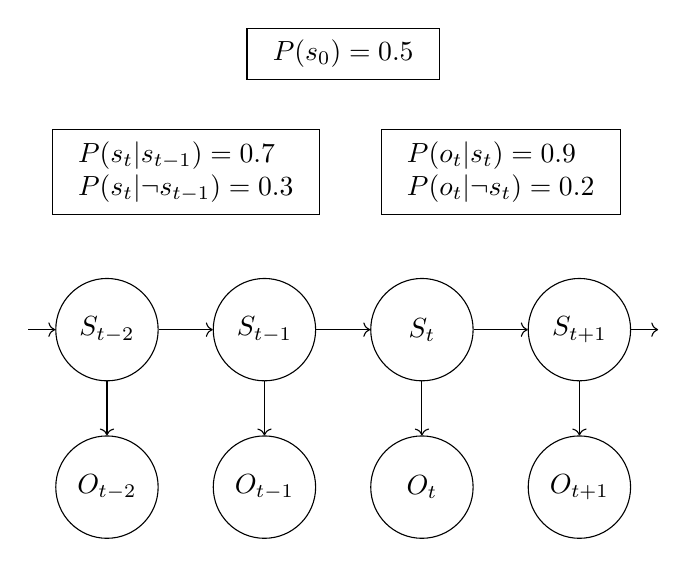
\begin{tikzpicture}[state/.style={circle, draw, minimum size=1.3cm}]

\node[draw] (tab1) at (3,7.5) {
\begin{tabular}{l}
$P(s_0) =0.5$ 
\end{tabular}
};

\node[draw] (tab2) at (1,6) {
\begin{tabular}{l}
$P(s_t | s_{t-1}) =0.7$ \\
$P(s_t | \neg s_{t-1}) =0.3$
\end{tabular}
};

\node[draw] (tab3) at (5,6) {
\begin{tabular}{l}
$P(o_t | s_t) =0.9$ \\
$P(o_t | \neg s_t) =0.2$
\end{tabular}
};

\node[state] (a) at (0, 4) {$S_{t-2}$};
\coordinate[left of=a] (d1);
\node[state] (b) at (2, 4) {$S_{t-1}$};
\node[state] (c) at (4, 4) {$S_{t}$};
\node[state] (d) at (6, 4) {$S_{t+1}$};
\coordinate[right of=d] (d2);
\path[draw] [->] (d1) -- (a);
\path[draw] [->] (a) -- (b);
\path[draw] [->] (b) -- (c);
\path[draw] [->] (c) -- (d);
\path[draw] [->] (d) -- (d2);

\node[state] (e) at (0, 2) {$O_{t-2}$};
\node[state] (f) at (2, 2) {$O_{t-1}$};
\node[state] (g) at (4, 2) {$O_{t}$};
\node[state] (h) at (6, 2) {$O_{t+1}$};
\path[draw] [->] (a) -- (e);
\path[draw] [->] (b) -- (f);
\path[draw] [->] (c) -- (g);
\path[draw] [->] (d) -- (h);

\end{tikzpicture}
\end{center}

\subsection*{The Full Robot Environment}

Let's consider a robot localization problem. This problem is similar to the example on page 389 of the Artificial Intelligence: Foundations of Computational Agents book by Poole and Mackworth.

\begin{figure}[ht!]
    \centering
    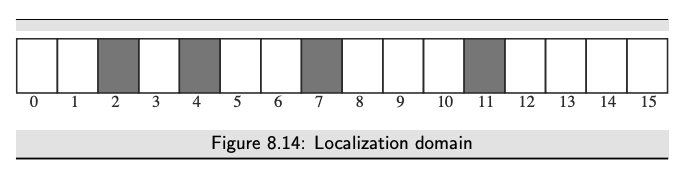
\includegraphics[scale=0.6]{images_posted/robot_localization.png}
    \caption{The Robot Localization Problem (from the Poole and Mackworth Textbook)}
    \label{fig:robot_localization_corridor}
\end{figure}

There is a circular corridor with $16$ locations numbered $0$ to $15$. There are doors at positions $2$, $4$, $7$, and $11$. There is no door at any other location. 

There is an arbitrary number of time steps, starting at time step $t = 0$. At each time step, the robot is at one of the $16$ locations. Let $S_t \in \{0, 1, \dots, 15\}$ denote the robot's location at time step $t$.

The robot's sensor noisily observes whether it is in front of a door or not. Let $O_t \in \{0, 1\}$ denote the robot's observation at time step $t$. $O_t = 0$ if the robot observes a door and $O_t = 1$ if the robot does not observe a door. The observation probabilities are given below.
%
\begin{align}
P(O_t = 0 | S_t \in \{2, 4, 7, 11\} ) & = 0.8 \\
P(O_t = 0 | S_t \not\in \{2, 4, 7, 11\} ) & = 0.1 
\end{align}

At each time step, the robot can choose one of three actions: move left, move right, and stay still. Let $A_t \in \{0, 1, 2\}$ denote the robot's action at time step $t$. $A_t = 0$ denotes moving left, $A_t = 1$ denotes moving right, and $A_t = 2$ denotes staying still. Taking an action may cause the robot to stay in the same location or move to a different location. The effects of the three actions are shown below.

The effects of moving left at time $t$:
%
\begin{align}
P(S_{t+1} = x | A_t = 0\land S_t = x) & = 0.05\\    
P(S_{t+1} = x - 1 \,(\text{mod } 16) | A_t = 0 \land S_t = x) & = 0.90\\    
P(S_{t+1} = x - 2 \,(\text{mod } 16)| A_t = 0 \land S_t = x) & = 0.05
\end{align}

The effects of moving right at time $t$:
\begin{align}
P(S_{t+1} = x | A_t = 1\land S_t = x) & = 0.15\\    
P(S_{t+1} = x + 1 \,(\text{mod } 16) | A_t = 1 \land S_t = x) & = 0.70\\    
P(S_{t+1} = x + 2 \,(\text{mod } 16)| A_t = 1 \land S_t = x) & = 0.15  
\end{align}

The effects of staying still at time $t$:
\begin{align}
P(S_{t+1} = x | A_t = 2\land S_t = x) & = 1.0
\end{align}

The environment has the following properties:
\begin{itemize}

\item The robot's observation at time $t$ depends only on the robot's location at time $t$. That is, for each $t$, $O_t$ depends on $S_t$ only.

\item The robot's location at time $t + 1$ only depends on its location at time $t$ and its action at time $t$. That is, for each $t$, $S_{t+1}$ depends on $S_t$ and $A_t$ only. 
\end{itemize}

The robot starts at an unknown location. At any time step, the robot tries to determine its location by estimating the probability of being in each location given its past observations and past actions. 





\newpage
\section{Locating the Robot by VEA (24 marks)}

You will calculate some probabilities for a simplified robot localization problem by executing the variable elimination algorithm.

{\bf The Simplified Robot Localization Problem: }

The circular corridor has 2 locations (0, 1). There is no door at location 0 and a door at location 1. The observation probabilities are as follows.
\begin{align}
& P(O_t = 0 | S_t = 1) = 0.8 \\
& P(O_t = 0 | S_t = 0) = 0.1 
\end{align}

The robot still has three actions, but the dynamics of the actions are simplified. 

The effects of moving left at time $t$:
\begin{align}
P(S_{t+1} = x | A_t = 0\land S_t = x) & = 0.05 \\    
P(S_{t+1} = x - 1 \,(\text{mod } 2) | A_t = 0 \land S_t = x) & = 0.95
\end{align}

The effects of moving right at time $t$:
\begin{align}
P(S_{t+1} = x | A_t = 1\land S_t = x) & = 0.15 \\    
P(S_{t+1} = x + 1 \,(\text{mod } 2) | A_t = 1 \land S_t = x) & = 0.85
\end{align}

The effects of staying still at time $t$:
\begin{align}
P(S_{t+1} = x | A_t = 2\land S_t = x) & = 1.0
\end{align}

We will represent this problem for three time steps (0 to 2) using the graphical model in Figure~\ref{fig:robot_localization_simple}.  

{\bf An important note regarding the actions: } The only purpose of observing the action at each time step is to determine the transition probabilities. We do not need to model the actions explicitly since they are not really random variables. For this reason, we have put the actions into the states for the time steps $0$ and $1$.

% In Figure~\ref{fig:robot_localization_simple_1}, we have nodes for the actions $A_0$ and $A_1$ similar to the nodes for the locations and observations. However, note that the actions are not really random variables. For our probabilistic inference problem, we will observe the robot's action in each time step. The only purpose of observing the actions is to determine the transition probabilities for the location $S_t$ to $S_{t+1}$ for any time step $t$. Let us simplify our graphical model by removing the nodes for the actions. Imagine that $A_t$ has been stored as part of $S_t$. For each $S_t$, we can use $A_t$ to derive the transition probabilities from $S_t$ to $S_{t+1}$. See Figure~\ref{fig:robot_localization_simple_2} for the simpler model.

\begin{figure}[ht!]
\centering
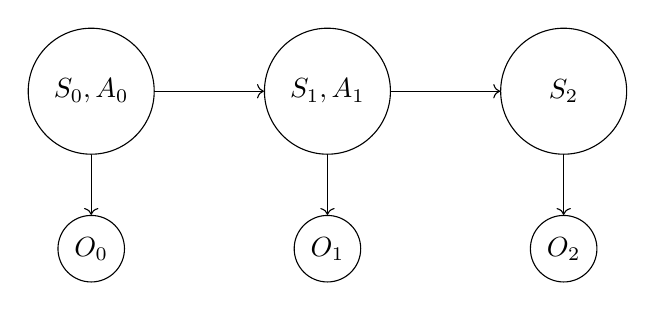
\begin{tikzpicture}

\node[draw, circle,minimum size=1.6cm] (a) at (0, 4) {$S_0, A_0$};
\node[draw, circle,minimum size=1.6cm] (b) at (3, 4) {$S_1, A_1$};
\node[draw, circle,minimum size=1.6cm] (c) at (6, 4) {$S_2$};
\path[draw] [->] (a) -- (b);
\path[draw] [->] (b) -- (c);

\node[draw, circle] (e) at (0, 2) {$O_0$};
\node[draw, circle] (f) at (3, 2) {$O_1$};
\node[draw, circle] (g) at (6, 2) {$O_2$};
\path[draw] [->] (a) -- (e);
\path[draw] [->] (b) -- (f);
\path[draw] [->] (c) -- (g);

\end{tikzpicture}

\caption{A Graphical Model of Simplified Robot Localization}
\label{fig:robot_localization_simple}
\end{figure}

{\bf Please answer the following questions.}

Using the Bayesian network in Figure~\ref{fig:robot_localization_simple}, answer the questions below by executing the variable elimination algorithm. 

\begin{enumerate}[(a)]
\item 
\label{q1_filtering}
Answer the question below by executing the variable elimination algorithm using the provided information. 
Eliminate the hidden variables in {\bf lexicographical order} \\
($S_0, S_1, S_2, O_0, O_1, O_2$). 

{\bf Please provide the final answer only. Make sure that your answer has 4 decimal places.}

\begin{problem}
At $t=2$, what is the probability that the robot is in location $0$? 

You can use the information below.
\begin{itemize}
    \item At $t=0$, the robot's prior belief over the two locations is a uniform distribution. That is, $P(S_0 = 0) = 0.5$ and $P(S_0 = 1) = 0.5$.
    \item At $t=0$, the robot does not observe the door and decides to move right, 
    \item At $t=1$, the robot observes the door and decides to move left.
    \item At $t=2$, the robot observes the door.
\end{itemize}

\end{problem}



\begin{markscheme}
(2 marks) Correct answer up to 3 decimal places. All or nothing.

\end{markscheme}


\item
\label{q1_smoothing}
Answer the question below by executing the variable elimination algorithm using the provided information. 
Eliminate the hidden variables in {\bf lexicographical order} \\
($S_0, S_1, S_2, O_0, O_1, O_2$). 

{\bf Please provide the final answer only. Make sure that your answer has 4 decimal places.}

\begin{problem}
At $t=1$, what is the probability that the robot is in location $0$? 

You can use the information below.
\begin{itemize}
    \item At $t=0$, the robot's belief over the two locations is a uniform distribution. That is, $P(S_0 = 0) = 0.5$ and $P(S_0 = 1) = 0.5$.
    \item At $t=0$, the robot does not observe the door and decides to move right, 
    \item At $t=1$, the robot observes the door and decides to move left.
    \item At $t=2$, the robot observes the door.
\end{itemize}

\end{problem}

\begin{markscheme}
(2 marks) Correct answer up to 3 decimal places. All or nothing.

\end{markscheme}


\item
\label{q1_general}
Answer the question below by executing the variable elimination algorithm using the provided information. 
Eliminate the hidden variables in {\bf lexicographical order} \\
($S_0, S_1, S_2, O_0, O_1, O_2$). 

{\bf Show all the steps of executing the variable elimination algorithm based on the formats in section~\ref{sec:vea_steps}}. {\bf Make sure that your final answer has 4 decimal places.}

\begin{problem}
At $t=1$, what is the probability that the robot is in location $0$ and does not observe a door? 

You can use the information below.
\begin{itemize}
    \item At $t=0$, the robot's belief over the two locations is a uniform distribution.  That is, $Pr(S_0 = 0) = 0.5$ and $Pr(S_0 = 1) = 0.5$.
    \item At $t=0$, the robot observes a door and decides to move right.
    \item At $t=1$, the robot decides to move left.
    \item At $t=2$, the robot does not observe the door.
\end{itemize}
\end{problem}


\begin{markscheme}
(20 marks)

\begin{itemize} 
\item
(2 marks) Correct answer up to 3 decimal places.
\item 
(18 marks) The algorithm execution has the correct steps.
\end{itemize}

\end{markscheme}



\end{enumerate}



\newpage
\subsection{Showing the execution steps of VEA}
\label{sec:vea_steps}

Please describe the steps of the variable elimination algorithm using the format specified below. You do not have to follow the spacing exactly. We will mark the steps by hand.

\begin{enumerate}

\item 
Show a factor as \verb+f(A B E)+. Use \verb+f+ to denote the name of every factor. Show the variables in {\bf lexicographical order}. For example,
%
\begin{verbatim}
f(A B E)
\end{verbatim}

\item 
After each operation (restrict, multiply, sum out, normalize), show the resulting factor in a table. The columns and rows can be in any order. For example,
%
\begin{verbatim}
 B,   E,   Prob
 True,  True,  0.9600
 True,  False,  0.9500
 False,  True,  0.2000
 False,  False,  0.0100
\end{verbatim}


\item 
Describe the {\bf define} operation as shown below. Show the factors in any order.
%
\begin{verbatim}
Define factors f(A G) f(A W)
\end{verbatim}

\item
Describe the {\bf restrict} operation as shown below.  
\begin{verbatim}
Restrict f(B E) to B = True to produce f(E)
 E,   Prob
 True,  0.9600
 False,  0.9500
\end{verbatim}

If you need to perform the restrict operation on multiple factors and on multiple variables for each factor, go through the factors in {\bf lexicographical order}. For each factor, go through the variables in {\bf lexicographical order}. Show one operation per line. 

The example below performs two restrict operation on \verb+f(A B E)+, one restrict operation on \verb+f(A G)+, and one restrict operation on \verb+f(A W)+.
%
\begin{verbatim}
Restrict f(A B E) to A = True to produce f(B E)
 B,   E,   Prob
 True,  True,  0.9600
 True,  False,  0.9500
 False,  True,  0.2000
 False,  False,  0.0100

Restrict f(B E) to B = True to produce f(E)
 E,   Prob
 True,  0.9600
 False,  0.9500

Restrict f(A G) to A = True to produce f(G)
 G,   Prob
 True,  0.4000
 False,  0.6000

Restrict f(A W) to A = True to produce f(W)
 W,   Prob
 True,  0.8000
 False,  0.2000

\end{verbatim}

\item
Describe the {\bf multiply} operation as shown below.
%
\begin{verbatim}
Multiply f(A B E) f(B) to produce f(A B E)
\end{verbatim}

If you need to multiply more than two factors together, show the operation on a single line. The factors can be in any order. For example,
%
\begin{verbatim}
Multiply f(E) f() f(E) f() f() to produce f(E)
 E,   Prob
 True,  0.0000
 False,  0.0001
\end{verbatim}

\item
Describe the {\bf sum out} operation as shown below.
%
\begin{verbatim}
Sum out W from f(W) to produce f()
Prob
1.0
\end{verbatim}

\item
Describe the {\bf normalize} operation as shown below.
%
\begin{verbatim}
Normalize f(E) to produce f(E)
 E,   Prob
 True,  0.0003
 False,  0.9997
\end{verbatim}

\end{enumerate}

See below for an example output for the Holmes network minus the node R. The network is given in lecture 13.

\begin{verbatim}
Computing P(E | A and B)

Define factors  f(A B E) f(A G) f(A W) f(B) f(E)

Restrict f(A B E) to A = True to produce f(B E)
 B,   E,   Prob
 True,  True,  0.9600
 True,  False,  0.9500
 False,  True,  0.2000
 False,  False,  0.0100

Restrict f(B E) to B = True to produce f(E)
 E,   Prob
 True,  0.9600
 False,  0.9500

Restrict f(A G) to A = True to produce f(G)
 G,   Prob
 True,  0.4000
 False,  0.6000

Restrict f(A W) to A = True to produce f(W)
 W,   Prob
 True,  0.8000
 False,  0.2000

Restrict f(B) to B = True to produce f()
Prob
0.0001

Sum out G from f(G) to produce f()
Prob
1.0

Sum out W from f(W) to produce f()
Prob
1.0

Multiply f(E) f() f(E) f() f() to produce f(E)
 E,   Prob
 True,  0.0000
 False,  0.0001

Normalize f(E) to produce f(E)
 E,   Prob
 True,  0.0003
 False,  0.9997

P(E | A and B) is 0.0003031569373991451
\end{verbatim}



\newpage
\section{Locating the Robot via an HMM (55 marks)}

You will implement the forward-backward algorithm to perform inference in an hidden Markov model. 

We have provided two python files: \verb+utils_soln.py+ and \verb+fba.py+.  \verb+utils_soln.py+ contains all the provided functions. \verb+fbs.py+ contains empty function stubs for you to complete.

Section~\ref{sec:forward_backward_algorithm} describes the forward-backward algorithm. Section~\ref{sec:modeling_environment} describes how you can model an environment using the \verb+Environment+ object in \verb+utils_soln.py+. 


{\bf Please complete the following tasks.}

Implement the empty functions in \verb+fba.py+. Submit \verb+fba.py+ only on Marmoset.
    
\begin{markscheme}
(55 marks)

Unit tests:
\begin{itemize}
    \item \verb+create_observation_matrix+ \\
    (1 public test + 2 secret tests) * 1 mark = 3 marks
    
    \item \verb+create_transition_matrices+ \\
    (1 public test + 2 secret tests) * 1 mark = 3 marks
    
    \item \verb+forward_recursion+ \\
    (1 public test + 6 secret tests) * 2 marks = 14 marks
    
    \item \verb+backward_recursion+ \\
    (1 public test + 6 secret tests) * 3 marks = 21 marks
    
    \item \verb+fba+ \\
    (1 public test + 6 secret tests) * 2 marks = 14 marks
\end{itemize}
    
\end{markscheme}

\newpage
\subsection{The Forward-Backward Algorithm}
\label{sec:forward_backward_algorithm}

There are $t$ time steps in total, from $0$ to $t-1$. The algorithm makes use of both forward and backward recursion.

%%%%%%%%%%%%%%%%%%%%%%%%%%%%%%%%%%%%%%%%
%%% Forward Recursion
%%%%%%%%%%%%%%%%%%%%%%%%%%%%%%%%%%%%%%%%
{\bf Step 1 (Forward Recursion): } Given the observations from time $0$ to time $t - 1$, forward recursion calculates the values $f_{0:k} = P(S_k | o_{0:k} )$ for $0 \le k \le t - 1$ using the recurrence relation below. 
%
\begin{align}
    \text{Base case: } f_{0:0} & = \alpha \, P(o_0 | S_0) P(S_0) \\
    \text{ Recursive case: } f_{0:k} & = \alpha \, P(o_k | S_k) \, \sum_{s_{k-1}} \, P(S_k | s_{k-1}) \, f_{0:(k-1)},\quad (1 \le k \le t - 1) 
\end{align}

The \verb+forward_recursion+ function returns a 2D \verb+numpy+ array of shape ($t$, \text{number of states}). The vector at index $i$ where $0 \le i \le t - 1$ is the normalized vector $f_{0:i}$.

%%%%%%%%%%%%%%%%%%%%%%%%%%%%%%%%%%%%%%%%
%%% Backward Recursion
%%%%%%%%%%%%%%%%%%%%%%%%%%%%%%%%%%%%%%%%
{\bf Step 2 (Backward Recursion): } Given observations from time $0$ to time $t-1$, backward recursion calculates the values $b_{(k+1):(t-1)} = P(o_{(k+1):(t-1)} | S_{k})$ for $0 \le k \le t-1$ using the recurrence relation below.
%
\begin{align}
    \text{ Base case: } b_{t:t-1} & = \vec{1} \\
    \text{ Recursive case: } b_{(k+1):t-1} & = \alpha \sum_{s_{k+1}} P(o_k | s_k ) \, b_{(k+2):t-1} \, P(s_{k+1} | S_k ),\quad (0 \le k \le t-2) 
\end{align}

The \verb+backward_recursion+ function returns a 2D \verb+numpy+ array of shape ($t+1$, \text{number of states}). 
%
The vector at index $0$ is not used by the algorithm and can be an arbitrary vector (our tests will ignore this vector).
%
The vector at index $i$ where $1 \le i \le t$ is the normalized vector $b_{i:(t-1)}$.

{\bf Step 3 (Forward-Backward Algorithm): } Given the observations from time $0$ to time $t-1$, the forward-backward algorithm calculates the values $P(S_k | O_0, \dots, O_{t-1})$ for $0 \le k \le t-1$ using the equation below.
%
\begin{align}
P(S_k | O_0, \dots, O_{t-1}) = \alpha \, f_{0:k} \, b_{k+1:t-1}, \quad (0 \le k \le t - 1)
\end{align}

The \verb+fba+ function returns a 2D \verb+numpy+ array of shape ($t$, \text{number of states}). 
%
The vector at index $i$ where $0 \le i \le t-1$ is the normalized vector $P(S_i | O_0, \dots, O_{t-1})$.


\newpage
\subsection{Modeling the umbrella, robot, or another environment}
\label{sec:modeling_environment}

We can use the \verb+Environment+ object to model a variety of environment including the umbrella and robot environments. We highly recommend that you test your program using a variety of environments.

\subsubsection{Modeling states}

\begin{itemize}
    \item The state types. (\verb+num_state_types+, \verb+state_types+)
        
        The states have different types. The state type determines the probabilities of generating different observations.
        
        For each environment, we will specify the number of state types (\verb+num_state_types+) and a list of state types (\verb+state_types+).
        
        For example,
        \begin{itemize}
            \item The umbrella environment has 2 types of states: rain (type 0), or no rain (type 1). We can initialize it as follows.
            
            \verb+num_state_types = 2+
            
            \verb+state_types = [0, 1]+
            
            \item The robot environment has 2 types of states: has door (type 0) or does not have door (type 1). We can initialize it as follows.
            
            \verb+num_state_types = 2+
            
            \verb+state_types = [1, 1, 0, 1, 0, 1, 1, 0, 1, 1, 1, 0, 1, 1, 1, 1]+
            
        \end{itemize}

    \item The number of states. We do not need to specify the number of states explicitly. The number of states is set to be the length of \verb+state_types+.

    For example, 
        \begin{itemize}
            \item The umbrella environment has 2 states.
            \item The robot environment has 16 states.
        \end{itemize}         


\end{itemize}


\subsubsection{Modeling observation probabilities}

The state type determines the probabilities of generating different observations. If two states have the same type, they generate the observations with the same probabilities.
It is sufficient to specify the observation probabilities for each state type instead of for each state. 

The \verb+Environment+ object's attribute \verb+observe_matrix+ stores the observation probabilities. 

% To create \verb+observe_matrix+, we must define the number of observation types (\verb+num_observe_types+) and the observation probabilities (\verb+observe_probs+). Then, we can call \\ \verb+create_observation_matrix+ to create \verb+observe_matrix+ using \verb+observe_probs+.

To create \verb+observe_matrix+, we first define the number of observation types (\verb+num_observe_types+). We assume that the observation types are \verb+[0, 1, ..., num_observe_types - 1]+.

Next, we will define \verb+observe_probs+: the probabilities of generating each observation type for each state type. \verb+observe_probs+ is a 2D list. Entry $(i,j)$ in \verb+observe_probs+ specifies the probability of generating observation type $j$ by state type $i$.

For example, 
\begin{itemize}
\item 
For the umbrella environment, there are two observation types: has umbrella (type 0) and no umbrella (type 1).
%
\begin{verbatim}
num_observe_types = 2
observe_probs = [[0.9, 0.1], [0.2, 0.8]]
\end{verbatim}

\item 
For the robot environment, there are two observation types: observes door (type 0) and does not observe door (type 1).
%
\begin{verbatim}
num_observe_types = 2
observe_probs = [[0.8, 0.2], [0.1, 0.9]]
\end{verbatim}

\end{itemize}

Given \verb+num_observe_types+ and \verb+observe_probs+, you need to implement \\
\verb+create_observation_matrix+ to create \verb+observe_matrix+ using \verb+observe_probs+.

The \verb+observe_matrix+ is a 2D numpy array. Entry $(i,j)$ in the array specifies the probability of generating observation type $j$ in state $i$ (not state type $i$). All the values in each row should sum to $1$ since they represent a distribution of observation probabilities.

\subsubsection{Modeling transition probabilities}

State transitions occur for different reasons in different environments. In the umbrella environment, the state transitions follow a stochastic process that the agent cannot control. In the robot environment, the robot's action at each time step causes a state transition to occur. 

The \verb+Environment+ object's attribute \verb+transition_matrices+ defines the transition probabilities. To accommodate the two types of environments, we will create \verb+transition_matrices+ in two different ways.

{\em Creating \verb+transition_matrices+ for the umbrella environment}

In the umbrella environment, state transitions occur based on a stochastic process. We initialize the environment with \verb+action_effects = None+ and a valid \verb+transition_matrices+ attribute.

\verb+transition_matrices+ is a 3D numpy array. The entry $(i,j,k)$ represents the probability of transitioning from state $j$ to state $k$ given action $i$. Since the umbrella environment has no actions, we will assume that there is a single dummy action. Thus, \verb+transition_matrices+ is a list containing a single 2D numpy array in it. See an example below.

\begin{verbatim}
transition_matrices = [[[0.7, 0.3], [0.3, 0.7]]]
\end{verbatim}

{\em Creating \verb+transition_matrices+ for the robot environment}

In the robot environment, different actions cause different state transitions. We initialize the environment with a valid \verb+action_effects+ attribute and \verb+transition_matrices = None+. You need to implement \verb+create_transition_matrices+ to create \verb+transition_matrices+ using \verb+action_effects+.

\verb+action_effects+ is a list of dictionaries. The $i$-th dictionary represents the state transition probabilities as a result of executing the $i$-th action. See an example below.
%
\begin{verbatim}
action_effects[0] = {0: 0.1, -1: 0.8, -2: 0.1}
action_effects[1] = {0: 0.1, 1: 0.8, 2: 0.1}
action_effects[2] = {0: 1.0}
\end{verbatim}
%
The keys in the $i$-th dictionary are relative state offsets after taking action $i$. The state offsets are relative to the current state; they may be positive, negative or zero. For example, a state offset of $-2$ means that the target state is two locations to the left, and a state offset of $4$ means that the target state is four locations to the right. Since the environment is circular, there are many ways of specifying the relative state offsets. For examples, for the moving left action, two possible set of keys are $[0, -1, -2]$ and $[0, 14, 15]$. Make sure that your code handles all the cases (by computing modulo the number of states).


You need to implement \verb+create_transition_matrix+ to create \verb+transition_matrices+ by using \verb+action_effects+.  The \verb+transition_matrix+ is a 3D numpy array. The entry $(i,j,k)$ in the array specifies the probability of transitioning from state $j$ to state $k$ by taking the i-th action. All the values in the $(i,j)$-th list should sum to $1$ since they represent a distribution of transition probabilities.


\end{document}





























